%----------------------------------------------------------------------------
%
%	This template was created by
%		Christian Krieg <christian.krieg@alumni.tuwien.ac.at>
%
%	April 2018
%
%----------------------------------------------------------------------------
%
\documentclass[%
	a4paper,
]
{article}
%
%----------------------------------------------------------------------------
%
% Institution
%
%\institution{Institute of Computer Technology}

%
%----------------------------------------------------------------------------
%
% Use the 'Libertine' font type
%
\usepackage{libertine}
\usepackage[T1]{fontenc}
\usepackage[utf8]{inputenc}
%
%----------------------------------------------------------------------------
%
% Set page margins
%
\usepackage{geometry}
\geometry{%
	left   = 2cm,
	right  = 2cm,
	top    = 2cm,
	bottom = 2cm
}
%
%----------------------------------------------------------------------------
%
% Set line spacing
%
\usepackage{setspace}
\setstretch{1.2}
%
%----------------------------------------------------------------------------
%
% Set paragraph: No indentation, but include an empty line
%
\usepackage[parfill]{parskip}
%
%----------------------------------------------------------------------------
%
% Set justification in algorithms
%
\usepackage{ragged2e}
%
%----------------------------------------------------------------------------
%
% Use colors
%
\usepackage{xcolor}
\usepackage{colortbl}
%
%----------------------------------------------------------------------------
%
% Define a TODO and a DONE command
%
\newcommand{\todo}[1]{\textcolor{red}{#1}}
\newcommand{\done}[1]{}
%
%----------------------------------------------------------------------------
%
% Use glossaries
%
\usepackage{glossaries}
\makeglossaries
%
% Glossary entries
%
\newglossaryentry{fpga}{
	name = {FPGA},
	description = {Field-programmable gate array},
	text = {FPGA},
	first = {field-programmable gate array (FPGA)},
	plural = {FPGAs},
	firstplural = {field-programmable gate arrays (FPGAs)},
}
%
\newglossaryentry{trng}{
	name = {TRNG},
	description = {True-random number generator},
	text = {TRNG},
	first = {true-random number generator (TRNG)},
	plural = {TRNGs},
	firstplural = {true-random number generators (TRNGs)},
}
%
\newglossaryentry{bcd}{
  name={BCD},
  description={Binary-coded decimal},
  text={BCD},
  first={binary-coded decimal (BCD)},
}
%
\newglossaryentry{hdl}{
  name={HDL},
  description={Hardware description language},
  text={HDL},
  first={hardware description language (HDL)},
  plural={HDLs},
  firstplural={hardware description languages (HDLs)},
}

\newglossaryentry{dicl}{
  name={DIC-Lab},
  description={Course held at TU-Wien on applying digital design techniques},
  text={DIC-Lab},
  first={Digital-Integrated-Circuits Laboratory (DIC-Lab)},
}

\newglossaryentry{bbs}{
  name={BBS},
  description={Blum-Blum-Shub algorithm},
  text={BBS},
  first={Blum-Blum-Shub algorithm (BBS)},
}

\newglossaryentry{prng}{
  name={PRNG},
  description={Pseudo-random number generator (PRNG)},
  text={PRNG},
  first={pseudo-random number generator (PRNG)},
  plural={PRNGs},
  firstplural={pseudo-random number generators (PRNGs)},
}
\newglossaryentry{uart}{
  name={UART},
  description={Universal Asynchronous Receiver Transmitter (UART)},
  text={UART},
  first={Universal Asynchronous Receiver Transmitter (UART)},
  plural={UARTs},
  firstplural={Universal Asynchronous Receiver Transmitters (UARTs)},
}
\newglossaryentry{nist}{
  name={NIST},
  description={National Institute of Standards and Technology (NIST)},
  text={NIST},
  first={National Institute of Standards and Technology (NIST)},
  plural={UARTs},
  firstplural={National Institute of Standards and Technology (NISTs)},
}
%
\newglossaryentry{vhdl}{
  name={VHDL},
  description={Very-high-speed integrated circuits hardware description
		language},
  text={VHDL},
  first={very-high-speed integrated circuits hardware description
		language (VHDL)},
}
%
\newglossaryentry{mac}{
  name={MAC},
  description={Message authentication code},
  text={MAC},
  first={message authentication code (MAC)},
  plural={MACs},
  firstplural={message authentication codes (MACs)},
}
%
\newglossaryentry{rtl}{
  name={RTL},
  description={Register-transfer level},
  text={RTL},
  first={register-transfer level (RTL)},
}
%
%\newglossaryentry{}{
%  name={},
%  description={},
%  text={},
%  first={},
%  plural={},
%  firstplural={},
%}
%
%----------------------------------------------------------------------------
%
% Settings for citations and the bibliography
%
\usepackage[%
	backend     = biber,
	maxbibnames = 99,
	citestyle   = numeric,
	autocite    = plain,
%	autocite    = footnote,
%	citestyle   = verbose-ibid,
	giveninits=true,
]{biblatex}
\bibliography{bib/blake2}
%
%----------------------------------------------------------------------------
%
% For Pseudo code
%
\usepackage[ruled]{algorithm2e}
\renewcommand{\algorithmcfname}{ALGORITHM}
\SetAlFnt{\normalsize}
\SetAlCapFnt{\normalsize}
\SetAlCapNameFnt{\normalsize}
%\SetAlCapHSkip{0pt}
%\IncMargin{-\parindent}
%
%----------------------------------------------------------------------------
%
%	TikZ -- TikZ ist kein Zeichenprogramm
%

\usepackage{tikz}
\usepackage{tikz-timing}
\usepackage{etoolbox}
\usetikzlibrary{mindmap}
\usetikzlibrary{shapes}
\usetikzlibrary{arrows}
\usetikzlibrary{decorations}
\usetikzlibrary{shapes.symbols}
\usetikzlibrary{shapes.geometric}
\usetikzlibrary{shapes.multipart}
\usetikzlibrary{positioning}
\usetikzlibrary{patterns}
\usetikzlibrary{calc}
\usetikzlibrary{scopes}         % cf. pgfmanual p.66
\usetikzlibrary{chains}         % cf. pgfmanual p.284
\usetikzlibrary{fit}
\usetikzlibrary{matrix}
\usetikzlibrary{decorations}
\usetikzlibrary{circuits.logic}
\usetikzlibrary{circuits.logic.IEC}
\usetikzlibrary{shapes.gates.logic.IEC}
%\usetikzlibrary{circuits.logic.US}
%\usetikzlibrary{shapes.gates.logic.US}
\usetikzlibrary{circuits.ee}
\usetikzlibrary{circuits.ee.IEC}
\usetikzlibrary{backgrounds}
\usetikzlibrary{automata}
\usetikzlibrary{intersections}
\usetikzlibrary{plotmarks}
\usepgflibrary{fpu}
\usetikzlibrary{decorations.pathreplacing}
%
%----------------------------------------------------------------------------
%
% TikZ shapes
%  
	% D flip-flops (DFFs) and shift register
% Author: Martin Scharrer
%\documentclass[a4paper,landscape]{article}

%\usepackage{pgf,tikz}
%%%<
%\usepackage{verbatim}
%\usepackage[active,tightpage]{preview}
%\PreviewEnvironment{tikzpicture}
%\setlength\PreviewBorder{5pt}%
%%%>

%\begin{comment}
%:Title: D flip-flops and shift register
%
%Example of a custom node shape for drawing  D flip-flops. The shape is used to draw a serial shift
%register. 
%
%\end{comment}
%
%\usetikzlibrary{calc,arrows}
%\usepackage{amsmath}
%\usepackage[left=1cm,right=1cm]{geometry}
%\pagestyle{empty}

\makeatletter

% Data Flip Flip (DFF) shape
\pgfdeclareshape{dff}{
  % The 'minimum width' and 'minimum height' keys, not the content, determine
  % the size
  \savedanchor\northeast{%
    \pgfmathsetlength\pgf@x{\pgfshapeminwidth}%
    \pgfmathsetlength\pgf@y{\pgfshapeminheight}%
    \pgf@x=0.5\pgf@x
    \pgf@y=0.5\pgf@y
  }
  % This is redundant, but makes some things easier:
  \savedanchor\southwest{%
    \pgfmathsetlength\pgf@x{\pgfshapeminwidth}%
    \pgfmathsetlength\pgf@y{\pgfshapeminheight}%
    \pgf@x=-0.5\pgf@x
    \pgf@y=-0.5\pgf@y
  }
  % Inherit from rectangle
  \inheritanchorborder[from=rectangle]

  % Define same anchor a normal rectangle has
  \anchor{center}{\pgfpointorigin}
  \anchor{north}{\northeast \pgf@x=0pt}
  \anchor{east}{\northeast \pgf@y=0pt}
  \anchor{south}{\southwest \pgf@x=0pt}
  \anchor{west}{\southwest \pgf@y=0pt}
  \anchor{north east}{\northeast}
  \anchor{north west}{\northeast \pgf@x=-\pgf@x}
  \anchor{south west}{\southwest}
  \anchor{south east}{\southwest \pgf@x=-\pgf@x}
  \anchor{text}{
    \pgfpointorigin
    \advance\pgf@x by -.5\wd\pgfnodeparttextbox%
    \advance\pgf@y by -.5\ht\pgfnodeparttextbox%
    \advance\pgf@y by +.5\dp\pgfnodeparttextbox%
  }

  % Define anchors for signal ports
  \anchor{D}{
    \pgf@process{\northeast}%
    \pgf@x=-1\pgf@x%
    \pgf@y=.5\pgf@y%
  }
  \anchor{CLK}{
    \pgf@process{\northeast}%
    \pgf@x=-1\pgf@x%
    \pgf@y=-.66666\pgf@y%
  }
  \anchor{CE}{
    \pgf@process{\northeast}%
    \pgf@x=-1\pgf@x%
    \pgf@y=-0.33333\pgf@y%
  }
  \anchor{Q}{
    \pgf@process{\northeast}%
    \pgf@y=.5\pgf@y%
  }
  \anchor{Qn}{
    \pgf@process{\northeast}%
    \pgf@y=-.5\pgf@y%
  }
  \anchor{R}{
    \pgf@process{\northeast}%
    \pgf@x=0pt%
  }
  \anchor{S}{
    \pgf@process{\northeast}%
    \pgf@x=0pt%
    \pgf@y=-\pgf@y%
  }
  % Draw the rectangle box and the port labels
  \backgroundpath{
    % Rectangle box
    \pgfpathrectanglecorners{\southwest}{\northeast}
    % Angle (>) for clock input
    \pgf@anchor@dff@CLK
    \pgf@xa=\pgf@x \pgf@ya=\pgf@y
    \pgf@xb=\pgf@x \pgf@yb=\pgf@y
    \pgf@xc=\pgf@x \pgf@yc=\pgf@y
    \pgfmathsetlength\pgf@x{.75ex} % size depends on font size
    \advance\pgf@ya by \pgf@x
    \advance\pgf@xb by \pgf@x
    \advance\pgf@yc by -\pgf@x
    \pgfpathmoveto{\pgfpoint{\pgf@xa}{\pgf@ya}}
    \pgfpathlineto{\pgfpoint{\pgf@xb}{\pgf@yb}}
    \pgfpathlineto{\pgfpoint{\pgf@xc}{\pgf@yc}}
    \pgfclosepath

    % Draw port labels
    \begingroup
    \tikzset{flip flop/port labels} % Use font from this style
    \tikz@textfont

    \pgf@anchor@dff@D
    \pgftext[left,base,at={\pgfpoint{\pgf@x}{\pgf@y}},x=\pgfshapeinnerxsep]{\raisebox{-0.75ex}{D}}

%    \pgf@anchor@dff@CE
%    \pgftext[left,base,at={\pgfpoint{\pgf@x}{\pgf@y}},x=\pgfshapeinnerxsep]{\raisebox{-0.75ex}{CE}}

    \pgf@anchor@dff@Q
    \pgftext[right,base,at={\pgfpoint{\pgf@x}{\pgf@y}},x=-\pgfshapeinnerxsep]{\raisebox{-.75ex}{Q}}

%    \pgf@anchor@dff@Qn
%    \pgftext[right,base,at={\pgfpoint{\pgf@x}{\pgf@y}},x=-\pgfshapeinnerxsep]{\raisebox{-.75ex}{$\overline{\mbox{Q}}$}}
%
%    \pgf@anchor@dff@R
%    \pgftext[top,at={\pgfpoint{\pgf@x}{\pgf@y}},y=-\pgfshapeinnerysep]{R}
%
%    \pgf@anchor@dff@S
%    \pgftext[bottom,at={\pgfpoint{\pgf@x}{\pgf@y}},y=\pgfshapeinnerysep]{S}
    \endgroup
  }
}

% Key to add font macros to the current font
\tikzset{add font/.code={\expandafter\def\expandafter\tikz@textfont\expandafter{\tikz@textfont#1}}} 

% Define default style for this node
% \tikzset{flip flop/port labels/.style={font=\sffamily\scriptsize}}
%\tikzset{every dff node/.style={draw,minimum width=2cm,minimum 
%height=2.828427125cm,very thick,inner sep=1mm,outer sep=0pt,cap=round,add 
%font=\sffamily}}
\tikzset{flip flop/port labels/.style={font=\tiny}}
\tikzset{every dff node/.style={draw,minimum width=.75cm,minimum 
height=1cm,inner sep=1mm,outer sep=0pt,cap=round,font=\scriptsize}}

\makeatother

%\begin{document}
%
%\begin{tikzpicture}[font=\sffamily,>=triangle 45]
%  \def\N{7}  % Number of Flip-Flops minus one
%
%  % Place FFs
%  \foreach \m in {0,...,\N}
%    \node [shape=dff] (DFF\m) at ($ 3*(\m,0) $) {Bit \#\m};
%
%  % Connect FFs (Q1 with D1, etc.)
%  \def\p{0}  % Used to save the previous number
%  \foreach \m in {1,...,\N} { % Note that it starts with 1, not 0
%    \draw [->] (DFF\p.Q) -- (DFF\m.D);
%    \global\let\p\m
%  }
%
%  % Connect and label data in- and output port
%  \draw [<-] (DFF0.D) -- +(-1,0) node [anchor=east] {input} ;
%  \draw [->] (DFF\N.Q) -- +(1,0) node [anchor=west] {output};
%
%  % 'Reset' port label
%  \path (DFF0) +(-2cm,+2cm) coordinate (temp)
%    node [anchor=east] {reset};
%  % Connect resets
%  \foreach \m in {0,...,\N}
%    \draw [->] (temp) -| (DFF\m.R);
%
%  % 'Set' port label
%  \path (DFF0) +(-2cm,-2cm) coordinate (temp)
%    node [anchor=east] {set};
%  % Connect sets
%  \foreach \m in {0,...,\N}
%    \draw [->] (temp) -| (DFF\m.S);
%
%  % Clock port label
%  \path (DFF0) +(-2cm,-2.5cm) coordinate (temp)
%    node [anchor=east] {clock};
%  \foreach \m in {0,...,\N}
%    \draw [->] (temp) -| ($ (DFF\m.CLK) + (-5mm,0) $) --(DFF\m.CLK);
%
%  % Clock port label
%  \path (DFF0) +(-2cm,-3cm) coordinate (temp)
%    node [anchor=east] {clock enable};
%  \foreach \m in {0,...,\N}
%    \draw [->] (temp) -| ($ (DFF\m.CE) + (-7.5mm,0) $) --(DFF\m.CE);
%\end{tikzpicture}
%
%\end{document}

    \usepackage{pgfplots,siunitx}
    \usepackage{graphicx}
	\graphicspath{{fig/}}
	\usepackage[section]{placeins}
%
%----------------------------------------------------------------------------
%
% Use AMS math fonts
%
\usepackage{amsfonts}
\usepackage[sans]{dsfont}
%
%----------------------------------------------------------------------------
%
% Use multiple figures in one float
%
\usepackage{subcaption}
%
%----------------------------------------------------------------------------
%
% Use dummy text
%
\usepackage{lipsum}
%
%----------------------------------------------------------------------------
%
% Use extended list environments (e.g., 'inparaenum')
%
\usepackage{paralist}
%
%----------------------------------------------------------------------------
%
% Use listings
%
\usepackage{listings}

\lstdefinestyle{vhdl}
{
	language=VHDL,
  basicstyle=\linespread{1}\scriptsize\ttfamily\color{black},
  commentstyle=\scriptsize\itshape,
  escapeinside={(*@}{@*)},
  frame=single, numbers=left,
%  numbersep=5pt,
  xleftmargin=15pt,
  xrightmargin=5pt,
  numbersep=5pt,
  breaklines=true,
  moredelim=**[is][\ttfamily\bfseries\color{red}]{(*}{*)},
}

\lstdefinestyle{verilog}
{
	language=Verilog,
  basicstyle=\linespread{1}\scriptsize\ttfamily\color{black},
  commentstyle=\scriptsize\itshape,
  escapeinside={(*@}{@*)},
  frame=single, numbers=left,
%  numbersep=5pt,
  xleftmargin=15pt,
  xrightmargin=5pt,
  numbersep=5pt,
  breaklines=true,
  moredelim=**[is][\ttfamily\bfseries\color{red}]{(*}{*)},
}
%
%----------------------------------------------------------------------------
%
% Typeset pseudo code
%
\usepackage{syntax}
\usepackage{amssymb}
%----------------------------------------------------------------------------
%
% More options for boxes
%
\usepackage{realboxes}
%
% Command for vertical text in tabulars
%
\newcommand*\rot{\rotatebox{90}}
%
%----------------------------------------------------------------------------
%
\usepackage{makecell}
%
%----------------------------------------------------------------------------
%
% Package for logos (e.g., the BibTeX logo)
%
\usepackage{dtk-logos}
%
%----------------------------------------------------------------------------
%
% Use \textsubscript
%
\usepackage{fixltx2e}
%
%----------------------------------------------------------------------------
%
% More options for tabulars
%
\usepackage{array}
\usepackage{tablefootnote}
\usepackage{threeparttable}
%
%----------------------------------------------------------------------------
%
% Support long tables
%
\usepackage{longtable}
%
%----------------------------------------------------------------------------
%
% Use appendices
%
\usepackage[titletoc]{appendix}
%
%----------------------------------------------------------------------------
%
% Settings for hyperlinks
%
\usepackage{hyperref}
\hypersetup{%
	colorlinks = true,
	allcolors  = blue,
}
%

%
%----------------------------------------------------------------------------
%
% Use the cleverref package -- Load this package as the very last!
%
\usepackage{cleveref}
%
%----------------------------------------------------------------------------
%
% Document body
%
\begin{document}
%
%----------------------------------------------------------------------------
\begin{titlepage}

	\begin{center}

	
\includegraphics[height=2cm]{fig/logo-tu-bw.png}%
	\hfill{}%
	
\includegraphics[height=2cm]{fig/logo-ict.png}%
	

	\vspace{5em}


		\large
		Benedikt TUTZER\\
		Dinka MILOVANCEV\\
	

	\vspace{5em}

		Course on \\[1em]
		{\huge Digital Integrated Circuits Design}\\[1em]
		{\Large 384.088, Summer Term 2018} \\[2em]
		{\large Supervisors:\\[.5em]
			Christian Krieg, Martin Mosbeck, Axel Jantsch} \\[5em]

		\today
		\vspace{5em}

		{\Huge BLAKE2 cryptographic hash and message authentication code (MAC)}\\[2em]
		{\Large An implementation in VHDL}

		\vspace{3em}
	\end{center}


\begin{abstract}

We implemented \emph{BLAKE2b} and \emph{BLAKE2s} hash function as specified in
RFC 7693. We used state machines to implement \emph{BLAKE2}.
%the implementation was syntactically correct
%and synthesizable.
Functional correctness is verified by comparing the produced output to the
reference implementation given in C. Our test bench compares the output of our
entity with the reference hash value for the same message input and reports
the result to stdout. A minimal design for the Digilent NEXYS 4 DDR board was
developed to prove that the blake2 cores are synthesizable and work as expected.
% The \emph{BLAKE2b} hash function
%entity is to be used as a component of \emph{Argon2} memory hard function
%which should generate cryptographically secure keys from passwords as
%specified in \autocite{irtf-cfrg-argon2-03}. The \emph{Argon2} function should
%be implemented targeting \emph{Nexyx 4 DDR} board.
\end{abstract}
\end{titlepage}
%
%----------------------------------------------------------------------------
%
%\vspace*{27em}

Copyright (C) 2018 Christian Krieg, Benedikt Tutzer, Dinka Milovancev

This work was originally developed in the course ``Digital Integrated
Circuits Design'' held at the Institute of Computer Technology (ICT), Vienna
University of Technology (TU Wien). If you find this work useful, please
cite it using the following \BibTeX{ } entry:

\vspace{1em}

\begin{lstlisting}[%
%	language   = TeX,%
	breaklines = true,%
	basicstyle = \ttfamily\footnotesize,%
%	columns    = flexible,%
	keepspaces = true,
	frame      = single,%
]
@TechReport{Krieg2018,
  author      = {Christian Krieg and Benedikt Tutzer and Dinka Milovancev},
  title       = {BLAKE2 cryptographic hash and message authentication code (MAC) -- An implementation in VHDL},
  institution = {Institute of Computer Technology, Vienna University of Technology (TU Wien)},
  year        = {2018},
  type        = {techreport},
  address     = {Gusshausstrasse 27--29 / 384, 1040 Wien},
  month       = {June},
}
\end{lstlisting}

\vspace{3em}
Contact us:

\href{christian.krieg@alumni.tuwien.ac.at}{christian.krieg@alumni.tuwien.ac.at}

\vfill


\includegraphics[height=1.5cm]{fig/cc-large.png}

\includegraphics[height=1.5cm]{fig/by-large.png}


This documentation is licensed under the following license:
Attribution 4.0 International (CC BY 4.0)

\vspace{3em}

You are free to:

\begin{enumerate}
    \item Share --- Copy and redistribute the material in any medium or format
    \item Adapt --- Remix, transform, and build upon the material for any purpose,
			even commercially.
\end{enumerate}

This license is acceptable for Free Cultural Works.

The licensor cannot revoke these freedoms as long as you follow the license terms.

The entire license text is available at:
\href{https://creativecommons.org/licenses/by/4.0/legalcode}
	{https://creativecommons.org/licenses/by/4.0/legalcode}


\pagebreak
%
%----------------------------------------------------------------------------
%
\newgeometry{%
	left   = 3.5cm,
	right  = 3.5cm,
	top    = 2cm,
	bottom = 2cm
}
%
%----------------------------------------------------------------------------
%
%\section{Features}
%\label{sec:features}
%
%\todo{Include a table here that holds key information that is useful for a
%potential user! Such as a data sheet does.}
%
%The \emph{BLAKE2} hash function comes in two variants: \emph{BLAKE2b} for
%64-bit platforms and \emph{BLAKE2s} for smaller architectures.
%%
%We implemented both \emph{BLAKE2b} and \emph{BLAKE2s} based on RFC 7693~%
%\autocite{rfc7693}.	
%
%The cores provide the following features:
%
%\begin{enumerate}
%
%	\item{}
%
%\end{enumerate}
%
%----------------------------------------------------------------------------
%
\section{Usage}
\label{sec:usage}

\done{Put in here typical usage examples the can be copied/pasted and ready
to be used. I think it would be cool to have this for all the variants given
in \Cref{sec:resource-allocation}.}

The \emph{BLAKE2} hash function comes in two variants: \emph{BLAKE2b} for
64-bit platforms and \emph{BLAKE2s} for smaller architectures.
%
We implemented both \emph{BLAKE2b} and \emph{BLAKE2s} based on RFC 7693~%
\autocite{rfc7693}.	
%
\Cref{lst:usage} shows how the BLAKE2s core is instantiated. Instantiating
the BLAKE2b core is similar, just replace ``blake2s'' by ``blake2b''.

To create hashes from an arbitrarliy long message up to $2^{128}$ bytes,
split the message into chunks of \emph{BLOCK_SIZE} bytes. Apply
them to the \emph{message} port sequentially. Once the message is stable,
raise \emph{valid_in} for one clock cycle.

If a key shall be used, it has be be sent as first chunk, padded with zeroes.
The length of the key needs to be available at the \emph{key_len} port.

\emph{message_len} needs to be set to the number of bytes that are to be
hashed in total. This includes the additional chunk containing the key, so when
a key is used, the size of one complete chunk needs to be added to
\emph{message_len} (128 for BLAKE2b or 64 for BLAKE2s respectively).

The length of the hash can be chosen by setting
\emph{hash_len}.

After sending one chunk, wait for \emph{compress_ready} to be `HIGH' before
sending the next chunk. When the last chunk is sent, the input
\emph{last_chunk} needs to be set to `HIGH'. After the last chunk is
encoded, the output \emph{valid_out} is raised and the hash is available at the
\emph{hash} output.

\begin{lstlisting}[%
	language   = VHDL,%
	breaklines = true,%
	basicstyle = \ttfamily\footnotesize,%
%	columns    = flexible,%
%	keepspaces = true,
	tabsize    = 4,
	frame      = single,%
	caption    = {Usage example for the BLAKE2s core. Instantiating a BLAKE2b
								is similar.},
	label      = lst:usage
]
architecture behav of example is
	component blake2s is
		port (
			reset          : in  std_logic;
			clk            : in  std_logic;
			message        : in  std_logic_vector(64 * 8 - 1 downto 0);
			hash_len       : in  integer range 1 to 32;
			valid_in       : in  std_logic;
			message_len    : in  integer range 0 to 2147483647;
			compress_ready : out std_logic;
			last_chunk     : in  std_logic;
			valid_out      : out std_logic;
			hash           : out std_logic_vector(32 * 8 - 1 downto 0)
		);
	end component;
begin
	hash : blake2s
	port map (
		reset          => reset,
		clk            => clk,
		message        => message,
		valid_in       => valid_in,
		message_len    => message_len,
		hash_len       => hash_len,
		compress_ready => compress_ready,
		last_chunk     => last_chunk,
		valid_out      => valid_out,
		hash           => hash
	);
...
end behav;
\end{lstlisting}
%
%----------------------------------------------------------------------------
%
\section{User Interface}
\label{sec:user-interface}
%

\begin{figure}[h!]
	\centering
	\small
	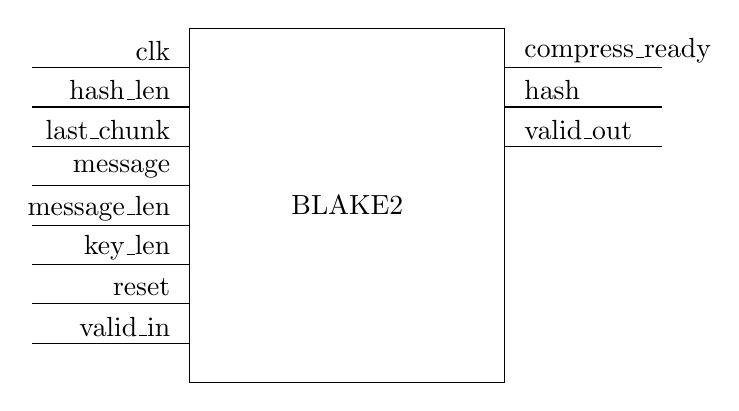
\begin{tikzpicture}[
	every node/.append style ={
		outer sep = 0,
		inner sep = 0,
	},
]

	\begin{scope}[anchor=east, every node/.append style={xshift=-.25cm, yshift=.6em}]
		\draw (0,0) -- (2,0) node {clk}; 
		\draw[yshift=-.5cm] (0,0) -- (2,0) node {hash\_len}; 
		\draw[yshift=-1cm] (0,0) -- (2,0) node {last\_chunk}; 
		\draw[yshift=-1.5cm] (0,0) -- (2,0) node {message}; 
		\draw[yshift=-2cm] (0,0) -- (2,0) node {message\_len};
		\draw[yshift=-2.5cm] (0,0) -- (2,0) node {key\_len};
		\draw[yshift=-3cm] (0,0) --  (2,0)node {reset}; 
		\draw[yshift=-3.5cm] (0,0) -- (2,0) node {valid\_in}; 
	\end{scope}

	\node (core) at (4,.5) [draw, anchor=north,inner sep=0, outer sep=0, minimum width=4cm, minimum height =4.5cm]{BLAKE2};

	\begin{scope}[anchor=west, every node/.append style={xshift=.25cm, yshift=.6em}]
		\draw (6,0) node {compress\_ready} --  (8,0); 
		\draw[yshift=-.5cm] (6,0) node {hash}  -- (8,0); 	
		\draw[yshift=-1cm] (6,0) node {valid\_out}  -- (8,0); 	
	\end{scope}

\end{tikzpicture}

	\caption{BLAKE2 entity}
	\label{fig:blake-entity}
\end{figure}

The functionality of BLAKE2s and BLAKE2b is encapsulated such that it is
transparent to the user to instantiate these cores. The ports to the
BLAKE2s and BLAKE2b cores are illustrated in \Cref{fig:blake-entity}.
\Cref{tbl:blake2-ports} lists the ports with additional information.

\begin{table}[htp]

	\centering
	\caption{Ports for the BLAKE2 cores}	
	\label{tbl:blake2-ports}
	\renewcommand{\arraystretch}{1.5}
	\begin{tabular}{l|c|c|m{3cm}}


	\hline
	\textbf{Port}
	& \textbf{Input/Output}
	&	\begin{minipage}[c]{3cm}%
				\textbf{Default value} \\
				(BLAKE2s/BLAKE2b)%
			\end{minipage}%
	& \textbf{Description}
	\\\hline

	clk
	& Input
	& ---
	& Clock signal
	\\\hline

	hash_len
	& Input
	& (32/64)
	&	Length of hash in bytes
	\\\hline

	last_chunk
	& Input
	& ---
	&	Signal to indicate that last message chunk is hashed%
	\\\hline

	message
	& Input
	& ---
	&	Input message to be hashed
	\\\hline

	message_len
	& Input
	& max. 2147483647
	& Total length of input message in bytes
	\\\hline

	key_len
	& Input
	& max. 128/64
	& Length of the key
	\\\hline

	reset
	& Input
	& ---
	& Reset signal
	\\\hline

	valid_in
	& Input
	& ---
	&	When `HIGH', data on the \emph{message} input is processed
	\\\hline

	hash
	& Output
	& ---
	&	The generated hash value
	\\\hline

	compress_ready
	& Output
	& ---
	&	When `HIGH', new data can be provided to the \emph{message} input
	\\\hline

	valid_out
	& Output
	& ---
	&	When `HIGH', the data at the \emph{hash} output is valid
	\\\hline

	\end{tabular}

\end{table}
%
%----------------------------------------------------------------------------
%
Internally, generics are used to switch between BLAKE2s and BLAKE2b
functionality. \Cref{tbl:blake2-generics} lists these generics along with
value range and default valuesfor BLAKE2s and BLAKE2b.

\begin{table}[tb]

	\centering
	\caption{Generics for the BLAKE2 cores}	
	\label{tbl:blake2-generics}
	\renewcommand{\arraystretch}{2}
	\begin{tabular}{l|c|c|m{3cm}}
	\hline
	\textbf{Name}
	& \textbf{Range}
	&	\begin{minipage}[c]{3cm}%
				\textbf{Default value} \\
				(BLAKE2s/BLAKE2b)%
			\end{minipage}%
	& \textbf{Description}
	\\\hline

	BASE_WIDTH
	& 32--64
	& 32/64
	& Width of the internal state vectors
	\\\hline

	COMP_ROUNDS
	& 1--64
	& 10/12
	&	Number of compression rounds to be used
	\\\hline

	BLOCK_SIZE
	& 1--512
	& 64/128
	&	Size of each message chunk
	\\\hline

	MAX_HASH_LENGTH
	& 1--2147483647
	& 32/64
	&	Maximum length of the hash
	\\\hline

	MAX_MESSAGE_LENGTH
	& 2147483647
	& 2147483647
	& Maximum length of input messages
	\\\hline

	\end{tabular}

\end{table}
%
%----------------------------------------------------------------------------
%
\section{Functional description}
\label{sec:implementation}

\done{Include a block diagram of the top-level entities here, ideally
created with TikZ.}

The \emph{BLAKE2} hash function comes in two variants: \emph{BLAKE2b} for
64-bit platforms and \emph{BLAKE2s} for smaller architectures.
%
We implemented both \emph{BLAKE2b} and \emph{BLAKE2s} based on RFC 7693~%
\autocite{rfc7693}.	
%
\Cref{fig:blake-entity} shows a block diagram of the BLAKE2 entity.
%
The input to \emph{BLAKE2} is the message data (message
length goes from 1 to $2^{128}$ bytes) and the output is the message digest or
simply hash value (hash length goes from 1 to 64 bytes).
%
According to the reference implementation~\autocite[16-26]{rfc7693}, the input message is
divided into $N$ 128 byte message blocks $m_i$; if a secret key is used, it is
used as the first message block. 
%
%In our design specification, the secret key is
%not used. \todo{Is it possible to enable key usage? This would be very cool,
%because then this core can be used to create \glspl{mac}.}
%
The hash value is iteratively computed as shown in \Cref{alg:bbs}.

\begin{algorithm}
\setstretch{1.2}
\justifying

	\ $h^{0}=IV$: Initialize the hash state vector with initialization
		vector $IV$. Obtain the $IV$ from the first 64 bits of the fractional
		parts of the first eight prime numbers' square roots. For creating
		a \gls{mac}, use a secret key instead.

	\BlankLine
	
    \For{$i:=0$ \textbf{to} $N-2$ }{

			$h^{i+1}$ $=$ compress($h_i, m_i,t_i,f=\textrm{`FALSE'} $)

			The
			compression function completely compresses one data block; it takes as
			an input the previous hash state, the current message block $m_i$ (divided
			into 16 words with length $w=64$ bits), $2 \cdot w$ bits wide offset counter
			$t_i$ that counts how many bytes have been compressed, and flag
			indicator $f$ for the last message block. The input message block is
			mixed into the current hash states.

		}

	\BlankLine
	

	$h^{N}$ $=$ ($h_{N-1}, m_{N-1},t_{N-1}$, $f=\textrm{`TRUE'} $) \

		Compute the final message block. The output is the first $hash\_len$
		bytes of little-endian state vector $h$. The input hash length parameter
		$hash\_len$ is in the range of 1 to 64 bytes.
		\done{This sentence is not quite clear to me... Is the information
		regarding $hash\_len$ relevant here?}

	\BlankLine

	\textbf{return $h^{N}$}
	
	\caption{\emph{BLAKE2b} algorithm}
	\label{alg:bbs}
	
\end{algorithm}

The main challenge in implementing the algorithm is the compression function
which is applied to each message block.
%
The message block is mixed in 10--12 rounds, and in each round, the message word
schedule is defined by 10 possible permutations $\sigma_0\dots\sigma_9$ (hard
coded into design as two dimensional \emph{SIGMA} array).
%
Mixing the messages requires an additional mixing function that mixes two
64-bit words from message $m_i$ into hash state $h_i$. We use an auxiliary
local $4\times{}4$ working vector $v[0..15]$ in the  mixing function:
\[
   v=
  \left[ {\begin{array}{cccc}
   v_0 & v_1 &v_2 & v_3 \\
   v_4 & v_5 &v_6 & v_7\\
   v_8 & v_9 &v_{10} & v_{11}\\
   v_{12} & v_{13} &v_{14} & v_{15}
  \end{array} } \right]
\]
	    
Hash functions are used in various security protocols to ensure the integrity
of transmitted data. Transmitted data is mapped to a hash value $h$ of fixed
size. It should be computationally impossible that two sets of data
result in the same hash value. Also, a small change in message data must
result in a large change in $h$, and it should be computationally impossible to
reconstruct the input data from the hash value.
%
We verify the quality of our \emph{BLAKE2b} implementation by comparing the
outputs to thte outputs produced by the reference implementation,
available as C code in RFC~7693~\autocite[16-26]{rfc7693}.

The \emph{BLAKE2b} hash algorithm is split into eight main operations which
are implemented as a state machine in \gls{vhdl}. The state machine implements
the following states (and state transitions):

\begin{enumerate}

	\item STATE_IDLE

		Initialize the \emph{BLAKE2b} hash function. Set initial values for the
		hash state vector $h[0..7]$ (array of 8 64-bit values). \done{If used as a
		hash function, use the pre-defined set of prime numbers' square roots.
		If used as a \gls{mac}, use a secret key instead, which is provided as
		input to the function.}
%
		If there is a new message block, set \emph{valid\_in} to
		`HIGH'. The next state is \mbox{STATE_PREPARE}. The counter which counts the
		number of compressed bytes (\emph{compressed\_bytes}) is incremented by
		the double base width (which is 128 for BLAKE2b). For the last message block,
		the \emph{compressed\_bytes} counter is set to the length of the message.

	\item STATE_PREPARE

		Initialize the compress function. Local state vector $v[0..15]$ is initialized
		with hash state vector $h[0..7]$, mixed with the number of received bytes.
		The counter which counts the number of mixing rounds \emph{ci_done} is reset
		to zero (there should be 10 or 12 rounds mixing a message). The next state is
		\mbox{STATE_COMPRESS}.

	\item STATE_COMPRESS

		Resets the counter for the mixing	function \emph{mi_done} to zero (its
		maximum	value is 7). The next state is the first mixing state,
		\mbox{STATE_MIX_A}. At the final mixing state \done{(which one is it? This
		is not quite clear to me...)},
		all the columns and diagonals of the working vector $v[0..15]$ are
		mixed with words of the current message block.

	\item STATE_MIX_A

		The first mixing state is one part of mixing function $G$ specified in
		RFC 7693~\autocite[7]{rfc7693}. $G$ requires word additions \done{(Does
		it mean to add words, or to perform the arithmetic operation `addition' on
		words?)}. In each cycle, one value of the working vector $v[0..15]$
		is computed depending on the \emph{SIGMA} permutation constant, the current
		mixing round, and the  2-bit wide tag \emph{mio_left} which serves
		to internally codify the mixing equations. The next mixing state is
		\mbox{STATE_MIX_B}.

	\item STATE_MIX_B

		The second mixing state implements the second part of mixing function $G$,
		and requires XOR operations and bit shifting. Again, in each cycle
		one value of the working vector $v[0..15]$ is computed depending on the
		\emph{SIGMA} permutation constant, the current mixing round, and internal
		the 2-bit wide tag \emph{mio\_left} to internally codify the mixing equations.

		\emph{mio\_left} is updated after each operation in state
		\mbox{STATE_MIX_B}.	If there are still pending mixing operations in a given
		round	(\emph{mi_done} $\neq 7$), then the next state is \mbox{STATE_MIX_A}.

		In total, there are eight mixing operations (\emph{mio_done}) divided into
		states $A$ and $B$ \done{(Hmmm, the term ``state'' seems to be used
		ambiguously here)}, and four operation codes for $AB$
		pairs. When all the	codes are computed in a given order, the counter which
		tracks the mixing code, \emph{mio\_left}, is incremented. If the last
		mixing operation is done but there are still mixing rounds pending, the next
		state is \mbox{STATE_COMPRESS}, and the counter that keeps track of the
		computed rounds, \emph{ci_done}, is updated.

		If all the mixing rounds are computed (\emph{ci_done} $= 11$), and the
		last message bit is sent ($seen\_last$ is `HIGH') the next state is
		\mbox{STATE_DONE}.

		If the last block is not yet sent but all the mixing
		rounds are already computed, the next state is \mbox{STATE_MIX_H}.

	\item STATE_MIX_H

		Mix the upper half $v[0..7]$ and the lower half $v[8..15]$ of the working
		vector $v[0..15]$ into the current state vector $h[0..7]$. The next state
		is \mbox{STATE_WAIT} to compress the next message block.

	\item STATE_WAIT

		Expect the next message block. If \emph{valid_in} goes `HIGH', the system
		variables are updated and the next state is \mbox{STATE_PREPARE}.

	\item STATE_DONE

		When the last message block has been compressed, the hash output is computed.
		The next state is \mbox{STATE_IDLE} in which we wait for the next message
		input.

\end{enumerate}		

\noindent
The state machine described above is implemented in \emph{blake2.vhd}.
%
%----------------------------------------------------------------------------
%
\section{Functional verification}
\label{sec:functional-verification}

In order to verify that the \emph{BLAKE2b} specification was correctly
implemented, we designed a test bench that reads input from a file
\emph{messages.txt} line by line.
%
Each line is hashed by the implemented algorithm. The same input
data is provided by the reference implementation in RFC 7693~%
\autocite{rfc7693}, which calculates the corresponding hash values. The
reference values are stored in the file \emph{hashes.txt}.
%
The test bench compares the output created by the design under test to
the reference values created by the reference implementation.
%

NOTE: In order to read the hash values from \emph{hashes.txt}, we need to
convert the values from hexadecimal to \emph{std_logic_vector}, wherefore
we define the function \emph{ASCII_2_STD} in the testbenches.

\Cref{fig:timing} shows the situation where a message block has been fully
compressed and a new message block is ready to be compressed (i.e., the round
counter \emph{ci_done} is `11', and the state is \mbox{STATE_WAIT}).
%
The BLAKE2 core signals this situation by setting \emph{valid_in} to `HIGH'
for one clock cycle.
%
Therefore, the next message block is written to \emph{current_chunk}, and the
next state is \mbox{STATE_PREPARE}. The message block register \emph{message}
is reset to zero when \emph{valid_in} is set to `LOW', and the state machine
enters \mbox{STATE_COMPRESS}.
%
Then \emph{mi_done} is reset to zero, and the BALKE2 core performs the mixing
function, visible in the \emph{state} variable (\mbox{STATE_MIX_A},
\mbox{STATE_MIX_B}). After the core performs the mixing, it updates the mixing
code signal \emph{mio\_left}.
%
Compressing of one 1024-bit message block consumes 835 clock cycles.

\begin{figure}[tb]
	\centering
	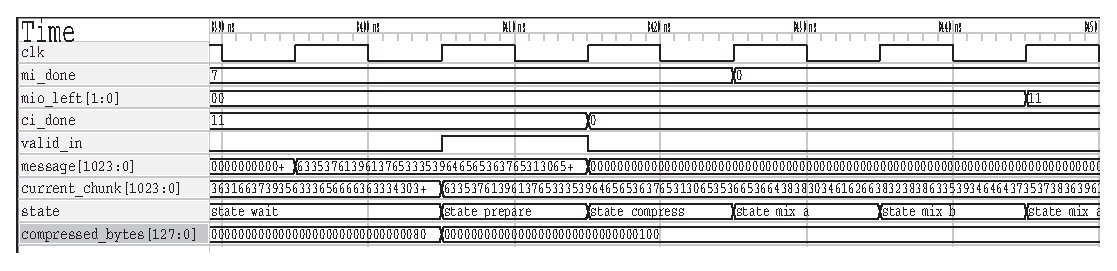
\includegraphics[width=\textwidth]{waveform2.eps};
	\caption{Simulation results for BLAKE2b hash function
		\done{Can we draw this in TikZ (using the TikZ timing package)? Adapting
			\Cref{fig:timing} may be the most straight-forward approach.}}
	\label{fig:timing}
\end{figure}
%
%\begin{figure}[tb]
%	\centering
%	\begin{tikztimingtable}
%		CLK & 30{ T } \\
%		$X$ & 15{D}{X} HHLLHHLLHHLLHHL \\
%		$O$ & 15{ L } HHLLHHLLHHLLHHL\\
%		$T$ & 15{ L } 15{H} \\
%	\extracode
%		\begin{pgfonlayer}{background}
%			\vertlines[black]{15}
%		\end{pgfonlayer}
%	\end{tikztimingtable}
%	\caption{Example timing diagram set in TikZ timing}
%	\label{fig:timing}
%\end{figure}

\Cref{tbl:blake2b-hashes} shows two example hashes for BLAKE2b. In order to
show that a small change in the message results in a large change in the hash,
we replaced one character of the original message (``\texttt{\footnotesize{}Message}''
vs. ``\texttt{\footnotesize{}Massage}''). \Cref{tbl:blake2s-hashes} shows the hash
values for the same input messages hashed with BLAKE2s.

\begin{table}[tb]
	\centering
	\caption{Example hashes and corresponding input messages for BLAKE2b}	
	\label{tbl:blake2b-hashes}
	\begin{tabular}{l|l|c}
	\hline
	\textbf{Input message} & \textbf{Hash value} & \textbf{Hash length} \\

	\hline
	\texttt{\footnotesize{}Message}
	& \makecell[lc]{%
		\texttt{\footnotesize{}24} \\
	}
	& 1 byte \\

	\hline
	\texttt{\footnotesize{}Message}
	& \makecell[lc]{%
		\texttt{\footnotesize{}2120} \\
	}
	& 2 bytes \\

	\hline
	\texttt{\footnotesize{}Message}
	& \makecell[lc]{%
		\texttt{\footnotesize{}0d93575d} \\
	}
	& 4 bytes \\

	\hline
	\texttt{\footnotesize{}Message}
	& \makecell[lc]{%
		\texttt{\footnotesize{}184c2242 418d7bc6} \\
	}
	& 8 bytes \\

	\hline
	\texttt{\footnotesize{}Message}
	& \makecell[cc]{%
		\texttt{\footnotesize{}ea30fef5 179fa367 0595e817 933e0ce8} \\
	}
	& 16 bytes \\

	\hline
	\texttt{\footnotesize{}Message}
	& \makecell[cc]{%
		\texttt{\footnotesize{}8a5efe6b 0c5a8d56 304804e8 aecfae16} \\
		\texttt{\footnotesize{}2e3799dc 92ad1942 b4bd72c5 2a97f3bd} \\
	}
	& 32 bytes \\

	\hline
	\texttt{\footnotesize{}Message}
	& \makecell[cc]{%
		\texttt{\footnotesize{}547ee071 8a19d53f df9f6123 8f31c139} \\
		\texttt{\footnotesize{}1979e95a 191505ba aa821805 1c4702d6} \\
		\texttt{\footnotesize{}f95d4312 d5c268f0 c6b4aa98 787dd91e} \\
		\texttt{\footnotesize{}3296ea3c d6d94833 fdfd5bae 39656b3c} \\
	}
	& 64 bytes \\

	\hline
	\texttt{\footnotesize{}Massage} &
	\makecell[cc]{%
		\texttt{\footnotesize{}566cb134 f53e14f2 7b49fcf5 45f4c71c} \\
		\texttt{\footnotesize{}4486c824 c0fe5359 c61df882 d610c38e} \\
		\texttt{\footnotesize{}88b25a1a 3e5790c4 b0099c9f 55f0ebc6} \\
		\texttt{\footnotesize{}71cf2aec 4a9b9134 d3f05b9e 8eee1612} \\
	}
	& 64 bytes \\

	\hline
	\texttt{\footnotesize{}abc}
	& \makecell[cc]{%
		\texttt{\footnotesize{}ba80a53f 981c4d0d 6a2797b6 9f12f6e9} \\
		\texttt{\footnotesize{}4c212f14 685ac4b7 4b12bb6f dbffa2d1} \\
		\texttt{\footnotesize{}7d87c539 2aab792d c252d5de 4533cc95} \\
		\texttt{\footnotesize{}18d38aa8 dbf1925a b92386ed d4009923} \\
	}
	& 64 bytes \\

	\hline
	\end{tabular}

\end{table}
%
%----------------------------------------------------------------------------
%
\begin{table}[tb]
	\centering
		\caption{Example hashes and corresponding input messages for BLAKE2s}
	\label{tbl:blake2s-hashes}
	\begin{tabular}{l|l|l}
	\hline
	\textbf{Input message} & \textbf{Hash value} & \textbf{Hash length} \\
	\hline

	\texttt{\footnotesize{}Message}
	& \makecell[lc]{%
		\texttt{\footnotesize{}fb} \\
	}
	& 1 byte \\

	\hline
	\texttt{\footnotesize{}Message}
	& \makecell[lc]{%
		\texttt{\footnotesize{}46ce} \\
	}
	& 2 bytes \\

	\hline
	\texttt{\footnotesize{}Message}
	& \makecell[lc]{%
		\texttt{\footnotesize{}57c3d825} \\
	}
	& 4 bytes \\

	\hline
	\texttt{\footnotesize{}Message}
	& \makecell[lc]{%
		\texttt{\footnotesize{}4a690e84 7edb95d8} \\
	}
	& 8 bytes \\

	\hline
	\texttt{\footnotesize{}Message}
	& \makecell[cc]{%
		\texttt{\footnotesize{}6e5cca08 1ec78d57 2b50cd1e efd754d1} \\
	}
	& 16 bytes \\

	\hline
	\texttt{\footnotesize{}Message}
	& \makecell[cc]{%
		\texttt{\footnotesize{}94bb1d33 b1ae1a65 aa1dad9b ade6c30b} \\
		\texttt{\footnotesize{}14f6ba03 0b6ab5e5 c9756aba 26b77219} \\
	}
	& 32 bytes \\

	\hline
	\texttt{\footnotesize{}Massage} &
	\makecell[cc]{%
		\texttt{\footnotesize{}f153acb5 47c9d8a3 199c4820 3d488df4} \\
		\texttt{\footnotesize{}82cc5a21 e760251a b7f090b7 7bdf8b5f} \\
	}
	& 32 bytes \\

	\hline
	\texttt{\footnotesize{}abc}
	& \makecell[cc]{%
		\texttt{\footnotesize{}508c5e8c 327c14e2 e1a72ba3 4eeb452f} \\
		\texttt{\footnotesize{}37458b20 9ed63a29 4d999b4c 86675982} \\
	}
	& 32 bytes \\

	\hline

	\end{tabular}

\end{table}

%Since this design is to be used as a module of the larger \emph{Argon2}
%design, there were no ports to be mapped to the hardware and therefore placing
%and routing of the design was not possible, but the RTL synthesis and
%optimization was successfully completed.
\Cref{RTLsynthesis} shows the \gls{rtl} optimization report.
%
%----------------------------------------------------------------------------
%
%\section{Formal verification}
%\label{sec:formal-verification}
%
%\todo{I put this here as a future point. Formal verification of a
%security-related core should be standard anyway. We should definitely teach
%that in next year's lab.}
%
%----------------------------------------------------------------------------
%

\section{Verification in Hardware}
A minimal design was developed to test the blake2b core in hardware. It is
available in the \emph{test\_top} subdirectory and can be synthesized using
Vivado targeting the Digilent Nexys DDR 4 board.\\
Communication to the core is given through the serial interface on the board,
allowing a host pc to send hash-requests to the internal blake2b core, which
will then respond by sending the requested hash back through the serial
interface. To request a hash, the following command needs to be issued by the
host pc:
\begin{center}
\emph{message\_len},\emph{hash\_len},\emph{key\_len},\emph{key},\emph{message}
\end{center}
where the parameters need to be chosen as follows:
\begin{itemize}
	\item \emph{message\_len}: The length of the message in byte
	\item \emph{hash\_len}: The length of the requested hash
	\item \emph{key\_len}: The length of the key to be used
	\item \emph{key}: The key to be used. The length of this field is given by
		\emph{key\_len}
	\item \emph{message}: The message to be used. The length of this field is given by
		\emph{message\_len}
\end{itemize}
Please note that there is no error handling, so the used must make sure that the
parameters that are sent to the board are inside the specifications of blake2b,
otherwise the behaviour is undefined.\\
The response from the board will be the raw binary representation of the hash
code. The result will be exactly as long as requested by the parameter
\emph{hash\_len}.

\section{Resource allocation}
\label{sec:resource-allocation}

%\todo{Here we should put tables for different targets (BLAKE2b, BLAKE2s with
%different bit widths) and hardware targets (Nexys and Ice40).}

\begin{lstlisting}[
	style = vhdl,
	caption = {RTL Hierarchical Component Statistics},
	label = {RTLsynthesis},
]
-
Hierarchical RTL Component report 
Module blake2b 
Detailed RTL Component Info : 
+---Adders : 
	   2 Input    128 Bit       Adders := 1     
	   3 Input     64 Bit       Adders := 1     
	   2 Input      4 Bit       Adders := 1     
	   2 Input      3 Bit       Adders := 1     
	   2 Input      2 Bit       Adders := 1     
+---XORs : 
	   2 Input     64 Bit         XORs := 5     
	   3 Input     64 Bit         XORs := 8     
+---Registers : 
	             1024 Bit    Registers := 1     
	              512 Bit    Registers := 1     
	              128 Bit    Registers := 1     
	               64 Bit    Registers := 24    
	               11 Bit    Registers := 1    
	                4 Bit    Registers := 1     
	                3 Bit    Registers := 2     
	                2 Bit    Registers := 1     
	                1 Bit    Registers := 3     
+---Muxes : 
	   8 Input    128 Bit        Muxes := 1     
	   2 Input    128 Bit        Muxes := 2     
	   3 Input     64 Bit        Muxes := 3     
	   8 Input     64 Bit        Muxes := 23    
	   4 Input     64 Bit        Muxes := 1     
	   9 Input     64 Bit        Muxes := 1     
	   8 Input      4 Bit        Muxes := 11    
	   8 Input      3 Bit        Muxes := 11    
	   2 Input      3 Bit        Muxes := 1     
	   3 Input      3 Bit        Muxes := 1     
	   8 Input      1 Bit        Muxes := 17    
	  11 Input      1 Bit        Muxes := 12    
	   4 Input      1 Bit        Muxes := 16    
	   2 Input      1 Bit        Muxes := 27    
----------------------------------------------
Finished RTL Hierarchical Component Statistics
----------------------------------------------

\end{lstlisting}
%
%----------------------------------------------------------------------------
%
\section{Additional notes}
\label{sec:additional-notes}

For the reference implementation given in RFC 7693~\autocite{rfc7693},
the input parameter is the whole message whose length can have between 1
and $2^{128}$ bytes.
%
This long message is intended to be divided into 128-byte message blocks
during hash computation. Since VHDL does not support such large input
vectors, we decided to send the message block by block.
%
This way, our data input is 128 bytes long, and we introduced additional
information regarding the message length (\emph{message_len} input).
%
%The maximum message length was specified to be 1032 bytes since this is the
%maximum length needed by \emph{Argon2}.\todo{Is this still valid?}
%
For every message block we need the information of the main module whether there
is a new message block available (signal \emph{valid_in} goes high) and the flag
register for the last message block \emph{last_chunk} (high if the last message
block is sent).
%
For the output we provide handshaking signals \emph{compress_ready}
and $valid\_out$, the user of our package must make sure that
\emph{compress_ready} is high before sending a new message block, and the
output hash can be stored when \emph{valid_out} is high.
%
The input messages in \texttt{messages.txt} file can be empty message. However
messages are not allowed to contain whitespace. \done{Why not? This is a very
strong constraint! We should definitely allow whitespace.}
%
%----------------------------------------------------------------------------
%
\section{Concluding remarks}
\label{sec:conclusding-remarks}

We implemented \emph{BLAKE2b} and \emph{BLAKE2s} hash algorithms in \gls{vhdl}.
The design is fully synthesizable. We functionally verified our design by
simulation. We used the reference implementation given in C in the original
specification of BLAKE2~\autocite{rfc7693} to verify that we correctly
implemented the algorithm. 
%On the ICE40 architecture, BLAKE2b consumes
%\todo{XYZ resources, running at a maximum clock of ZYX Hz}, and BLAKE2s
%onsumes \todo{from ABC to DEF resources, running at a maximum clock speed of
%GHI Hz}.
%
%----------------------------------------------------------------------------
%
% References
%
\printbibliography
%
%----------------------------------------------------------------------------
%

\end{document}
%
%----------------------------------------------------------------------------
